\chapter{Revisão de números complexos e funções trigonométricas} %Relação de Euler
\section{Funções trigonométricas}
\begin{defn}
Dado um número real $\theta$, $0\leq \theta<\frac{\pi}{2}$, seno de $\theta$ ($\sen(\theta)$) é definido pelo número real associado ao triângulo retângulo de ângulos $\theta$ rad, $\frac{\pi}{2}-\theta$ rad e $\frac{\pi}{2}$ rad como a razão do cateto oposto ao ângulo $\theta$ e a hipotenusa. O cosseno é a razão do cateto adjacente ao ângulo $\theta$ e a hipotenusa.
\end{defn}
\begin{defn}(Extensão das funções trigonométricas)
\begin{itemize}
\item[a)] Dado um número real $\theta$, $0\leq \theta<2\pi$, as funções trigonométricas são estendidas da seguinte forma:
\begin{eqnarray*}
\cos(\theta)&=&-\cos(\pi-\theta)\qquad \hbox{se }\ \theta\in \left(\frac{\pi}{2},\pi\right]\\
\sen(\theta)&=&\sen(\pi-\theta)\qquad \hbox{se }\ \theta\in \left(\frac{\pi}{2},\pi\right]\\
\cos(\theta)&=&-\cos(\theta-\pi)\qquad \hbox{se }\ \theta\in \left[\pi,\frac{3\pi}{2}\right)\\
\sen(\theta)&=&-\sen(\theta-\pi)\qquad \hbox{se }\ \theta\in \left[\pi,\frac{3\pi}{2}\right)\\
\cos(\theta)&=&\cos(2\pi-\theta)\qquad \hbox{se }\ \theta\in \left(\frac{3\pi}{2},2\pi\right]\\
\sen(\theta)&=&-\sen(2\pi-\theta)\qquad \hbox{se }\ \theta\in \left(\frac{3\pi}{2}2\pi\right]\\
\end{eqnarray*}
\item[b)] A extensão para todos os números reais se dá pela periodicidade:
\begin{eqnarray*}
\cos(\theta+2k\pi)&=&\cos(\theta),\ k\in\mathbb{Z}\\
\sen(\theta+2k\pi)&=&\sen(\theta),\ k\in\mathbb{Z}\\
\end{eqnarray*}
\end{itemize}
\end{defn}
\begin{defn}
Dado um número real $\theta$, $0\leq \theta<2\pi$, define-se tangente de $\theta$ por
\begin{eqnarray*}
\tan(\theta)&=&\frac{\sen(\theta)}{\cos(\theta)},\qquad \theta\neq \frac{\pi}{2}\ \hbox{e}\ \theta\neq \frac{3\pi}{2},\\
\end{eqnarray*}
secante de $\theta$ por
\begin{eqnarray*}
\sec(\theta)&=&\frac{1}{\cos(\theta)},\qquad \theta\neq \frac{\pi}{2}\ \hbox{e}\ \theta\neq \frac{3\pi}{2},\\
\end{eqnarray*}
cossecante de $\theta$ por
\begin{eqnarray*}
\csc(\theta)&=&\frac{1}{\sen(\theta)},\qquad \theta\neq 0\ \hbox{e}\ \theta\neq \pi\\
\end{eqnarray*}
e
cotangente de $\theta$ por
\begin{eqnarray*}
\cot(\theta)&=&\frac{\cos(\theta)}{\sen(\theta)},\qquad \theta\neq 0\ \hbox{e}\ \theta\neq \pi.\\
\end{eqnarray*}
\end{defn}
\begin{prop} Dado $x,\ y\in \mathbb{R}$, valem as seguintes afirmações:
\begin{itemize}
\item[a)] $\sen^2(x)+\cos^2(x)=1$
\item[b)] $\sen(x+y)=\sen(x)\cos(y)+\sen(y)\cos(x)$
\item[c)] $\sen(x-y)=\sen(x)\cos(y)-\sen(y)\cos(x)$
\item[d)] $\sen(2x)=2\sen(x)\cos(x)$
\item[e)] $\cos(x+y)=\cos(x)\cos(y)-\sen(y)\sen(x)$
\item[f)] $\cos(x-y)=\cos(x)\cos(y)+\sen(y)\sen(x)$
\item[g)] $\cos(2x)=\cos^2(x)-\sen^2(x)$
\item[h)] $\tan(x+y)=\frac{\tan(x)+\tan(y)}{1-\tan(x)\tan(y)},\qquad x\neq \frac{\pi}{2}+k\pi,\ k\in\mathbb{Z}.$
\item[i)] As séries de Taylor do seno e cosseno são dadas por
$$\sen(x)=\sum_{k=0}^\infty\frac{(-1)^k x^{2k+1}}{(2k+1)!}=x-\frac{x^3}{3!}+\frac{x^5}{5!}-\cdots $$
$$\cos(x)=\sum_{k=0}^\infty\frac{(-1)^k x^{2k}}{(2k)!}=1-\frac{x^2}{2!}+\frac{x^4}{4!}-\cdots $$
\end{itemize}
\end{prop}
\section{Números complexos e fórmula de Euler}
\begin{defn} Um número complexo é definido pelo par ordenado $(a,b)$ de números reais que satisfazem as seguintes operações de adição e multiplicação:
\begin{eqnarray*}
(a_1,b_1)+(a_2,b_2)&=&(a_1+a_2,b_1+b_2)\\
(a_1,b_1)\cdot(a_2,b_2)&=&(a_1a_2-b_1b_2,a_1b_2+a_2b_1).
\end{eqnarray*}
O conjunto dos números complexos é denotado por $\mathbb{C}$.
\end{defn}
\begin{obs}(Números complexos)
\begin{itemize} 
\item[a)] Os números complexos da forma $(a,0)$ são identificados com os números reais $(a,0)\equiv a$.
\item[b)] O número complexo $(0,1)$ é chamado de unidade imaginária e denotada por $i$. Observe que $i^2=-1$
\item[c)] Os números complexos da forma $z=(a,b)$ são rotineiramente denotados na sua forma retangular por $z=a+bi$, onde $a$ é a parte real de $z$ (Re\ \!$(z)=a$ ) e $b$ é a parte imaginária de $z$ (Im\ \!$(z)=b$ ).
\item[d)] A representação geométrica do número $z=a+bi$ no plano complexo é dada por um plano cartesiano onde um eixo marca a parte real e o outro marca a parte imaginária (veja figura \ref{num_complexo}).
\end{itemize}
\end{obs}
\begin{defn}Dado um número complexo $z=a+bi$, definimos módulo de $z$ ($|z|$) por $|z|=\sqrt{a^2+b^2}$. Também definimos argumento $\theta$ para $z\neq 0$ como qualquer  solução do sistema
\begin{eqnarray}
 \cos(\theta)&=&\frac{a}{\sqrt{a^2+b^2}},\\
 \sin(\theta)&=&\frac{b}{\sqrt{a^2+b^2}}.
\end{eqnarray}
Observe que este sistema possui infinitas soluções. Ademais, se $\theta_1$ e $\theta_2$ são duas soluções, então diferem por um múltiplo inteiro de $2\pi$, isto é, $\theta_1-\theta_2=2n\pi$, $n$ inteiro.
\end{defn}
Observe que uma possível solução, com $-\frac{\pi}{2}<\theta\leq \frac{3\pi}{2}$ é dada por
$$
\theta=\left\{\begin{array}{cc}\tan^{-1}\left(\frac{b}{a}\right)&\hbox{se}\ a>0\\[5pt]
\frac{\pi}{2}&\hbox{se}\ a=0\ \hbox{e}\ b>0\\[5pt]
\frac{3\pi}{2}&\hbox{se}\ a=0\ \hbox{e}\ b<0 \\[5pt] 
\tan^{-1}\left(\frac{b}{a}\right)+\pi&\hbox{se}\ a<0\end{array}\right.
$$
Se desejamos $\frac{\pi}{2}\leq \theta < \frac{\pi}{2}$, podemos usar a seguinte expressão:
$$\theta=\begin{cases}
\tan^{-1}(\frac b a) &\text{se } a > 0, \\[5pt]
\tan^{-1}(\frac b a) + \pi &\text{se } a < 0 \text{ e } b \ge 0, \\[5pt]
\tan^{-1}(\frac b a) - \pi &\text{se } a < 0 \text{ e } b < 0, \\[5pt]
+\frac{\pi}{2} &\text{se } a = 0 \text{ e } b > 0, \\[5pt]
-\frac{\pi}{2} &\text{se } a = 0 \text{ e } b < 0, \\[5pt]
\end{cases}$$
A representação geométrica de $|z|$ e $\theta$ está na figura \ref{num_complexo}.
\begin{figure}[!ht]
\begin{center}

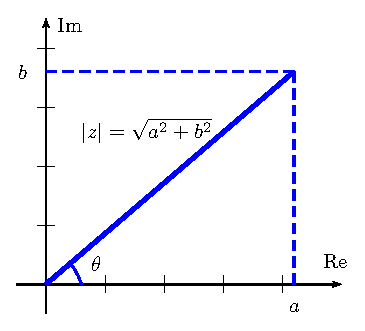
\includegraphics{cap_num_complexos/pics/figura_1}\end{center}
\caption{\label{num_complexo}}
\end{figure}
\begin{defn}A forma trigonométrica de um número complexo $z=a+bi$ é 
$$
z=|z|\left(\cos(\theta)+i\sen(\theta)\right),
$$
onde $|z|=\sqrt{a^2+b^2}$ é o módulo de $z$ e $\theta$ satisfazendo $a=|z|\cos(\theta)$ e $b=|z|\sen(\theta)$ é o argumento.
\end{defn}
\begin{ex}Para escrever o número $z=2-2i$ na forma trigonométrica, calculamos o módulo $|z|=\sqrt{2^2+(-2)^2}=2\sqrt{2}$ e o argumento, que satisfaz $\sen(\theta)=-\frac{2}{2\sqrt{2}}=-\frac{\sqrt{2}}{2}$ e $\cos(\theta)=\frac{2}{2\sqrt{2}}=\frac{\sqrt{2}}{2}$, ou seja, $\theta=\frac{7\pi}{4}$. Logo, $z=2\sqrt{2}\left(\cos\left(\frac{7\pi}{4}\right)+i\sen\left(\frac{7\pi}{4}\right)\right)$. 
\end{ex}
\begin{defn}Dado $z\in\mathbb{C}$, definimos exponencial de $z$ por
$$
e^z=1+z+\frac{z^2}{2!}+\frac{z^3}{3!}+\frac{z^4}{4!}+\cdots=1+\sum_{k=1}^\infty \frac{z^k}{k!}
$$
\end{defn}
\begin{prop}(Fórmula de Euler) Dado $\theta\in\mathbb{R}$, vale a identidade
$$
e^{i\theta}=\cos(\theta)+i\sen(\theta).
$$
\end{prop}
\begin{proof}
De fato,
\begin{eqnarray*}
e^{i\theta}&=&1+i\theta+\frac{(i \theta)^2}{2!}+\frac{(i\theta)^3}{3!}+\frac{(i\theta)^4}{4!}+\frac{(i\theta)^5}{5!}+\cdots\\
&=&1+i\theta-\frac{\theta^2}{2!}-i\frac{\theta^3}{3!}+\frac{\theta^4}{4!}+i\frac{\theta^5}{5!}+\cdots\\
&=&1-\frac{\theta^2}{2!}+\frac{\theta^4}{4!}+\cdots    +i\left(\theta-\frac{\theta^3}{3!}+\frac{\theta^5}{5!}+\cdots\right)\\
&=&\cos(\theta)    +i\sen(\theta)
\end{eqnarray*}
\end{proof}
\begin{defn}A forma exponencial de um número complexo $z=a+bi$ é 
$$
z=|z|e^{i\theta},
$$
onde $|z|=\sqrt{a^2+b^2}$ é o módulo de $z$ e $\theta$ satisfazendo $a=|z|\cos(\theta)$ e $b=|z|\sen(\theta)$ é o argumento.
\end{defn}
\begin{ex}Para escrever o número $z=2-2i$ na forma exponencial, calculamos o módulo $|z|=2\sqrt{2}$ e o argumento $\theta=\frac{7\pi}{4}$ e escrevemos $z=2\sqrt{2}e^{i\frac{7\pi}{4}}$. 
\end{ex}
\begin{prob}{\label{prob_sin_euler}}Mostre que
$$
\sen(\theta)=\frac{e^{i\theta}-e^{-i\theta}}{2i}
$$
e
$$
\cos(\theta)=\frac{e^{i\theta}+e^{-i\theta}}{2}
$$
\end{prob}
\begin{proof}
Observe que pela fórmula de Euler vale
\begin{equation}{\label{Euler_1}}
e^{i\theta}=\cos(\theta)+i\sen(\theta)
\end{equation}
e
\begin{equation}{\label{Euler_2}}
e^{-i\theta}=\cos(\theta)-i\sen(\theta).
\end{equation}
A diferença das equações (\ref{Euler_1}) e (\ref{Euler_2}) nos dá a expressão para o seno e a soma delas nos dá a expressão para o cosseno.
\end{proof}
\begin{ex}Para calcular $\cos^2(\theta)$ usando as expressões do problema \ref{prob_sin_euler} fazemos o seguinte:
\begin{eqnarray*}
\cos^2(\theta)&=&\left(\frac{e^{i\theta}+e^{-i\theta}}{2}\right)^2\\
&=&\frac{\left(e^{i\theta}\right)^2+2e^{i\theta}e^{-i\theta}+\left(e^{-i\theta}\right)^2}{4}\\
&=&\frac{2+e^{2i\theta}+e^{-2i\theta}}{4}\\
&=&\frac{1+\frac{e^{2i\theta}+e^{-2i\theta}}{2}}{2}\\
&=&\frac{1+\cos(2\theta)}{2}
\end{eqnarray*}
\end{ex}
\section{Exercícios}
\begin{Exercise}
Relacione $A$ e $\theta$ com os valores conhecidos de $B$ e $C$ que satisfazem a identidade
$$A\cos(x-\theta)=B\cos(x)+C\sen(x),~~~~\forall x\in\mathbb{R}$$
sabendo que $0\leq \theta<2\pi$ e $A\geq 0$.
\end{Exercise}
\begin{Answer}
$A=\sqrt{B^2+C^2}$ e $\theta$ satisfaz simultaneamente $\cos(\theta)=\frac{B}{\sqrt{B^2+C^2}}$ e $\sen(\theta)=\frac{C}{\sqrt{B^2+C^2}}$.
\end{Answer}
\begin{Exercise} Encontre $A$ e $\theta$ com $A\geq 0$ e  $0\leq \theta<2\pi$ tal que
\begin{itemize}
 \item [a)] $A\cos(x-\theta)=3\cos(x)+4\sen(x)$
 \item [b)] $A\cos(x-\theta)=3\cos(x)-4\sen(x)$
 \item [c)] $A\cos(x-\theta)=-3\cos(x)+4\sen(x)$
 \item [d)] $A\cos(x-\theta)=-3\cos(x)-4\sen(x)$
 \item [e)] $A\cos(x-\theta)=\sen(x)$
 \item [f)] $A\cos(x-\theta)=2\cos(x)$
 \item [g)] $A\cos(x-\theta)=-2\cos(x)$
 \end{itemize}
\end{Exercise}
\begin{Answer}
\begin{itemize}
 \item [a)] $A=5$, $\theta=\varphi$
 \item [b)] $A=5$, $\theta=2\pi-\varphi$
 \item [c)] $A=5$, $\theta=\pi-\varphi$
 \item [d)] $A=5$, $\theta=\pi+\varphi$
 \item [e)] $A=1$, $\theta=\frac{\pi}{2}$
 \item [f)] $A=2$, $\theta=0$
 \item [g)] $A=2$. $\theta=\pi$
 \end{itemize}
 onde $\varphi=\cos^{-1}\left(\frac{3}{5}\right)=\sen^{-1}\left(\frac{4}{5}\right)=\tan^{-1}\left(\frac{4}{3}\right)\approx 0.9272952rad $
\end{Answer}
\begin{Exercise}Escreva os seguintes números complexos na forma exponencial. Calcule também o complexo conjugado de cada um. Represente-os no plano complexo e identifique no gráfico as partes real e complexa, o argumento e o módulo.
\begin{itemize}
\item[a)] $2+3i$
\item[b)] $-2+3i$
\item[c)] $3-4i$
\item[d)] $-3-4i$
\item[e)] $4$
\item[f)] $5i$
\item[g)] $-5$
\item[h)] $-4i$
\end{itemize}
\end{Exercise}
\begin{Answer}
\begin{itemize}
\item[a)] $\sqrt{13}e^{i\theta}$, $\theta=\tan^{-1}\left(\frac{3}{2}\right)$
\item[b)] $\sqrt{13}e^{i\theta}$, $\theta=\pi-\tan^{-1}\left(\frac{3}{2}\right)$
\item[c)] $5e^{i\theta}$, $\theta=2\pi-\tan^{-1}\left(\frac{4}{3}\right)$
\item[d)] $5e^{i\theta}$, $\theta=\pi+\tan^{-1}\left(\frac{4}{3}\right)$
\item[e)] $4~~\left(4e^{0}\right)$
\item[f)] $5e^{i\frac{\pi}{2}}$
\item[f)] $5e^{i\pi}$
\item[g)] $4e^{i\frac{3\pi}{2}}$
\end{itemize}
\end{Answer}
\begin{Exercise}Escreva os seguintes números complexos na forma retangular. Represente-os no plano complexo e identifique no gráfico as partes real e complexa, o argumento e o módulo.
\begin{itemize}
\item[a)] $e^{5\pi i}$
\item[b)] $e^{3\pi i+2}$
\item[c)] $4e^{2\pi i}$
\item[d)] $2e^{\frac{\pi}{2}i+1}e^{-2}$
\item[e)] $4e^{-\frac{\pi}{4}i}$
\item[f)] $5e^{\frac{\pi}{4}i}$
\end{itemize}
\end{Exercise}
\begin{Answer}
\begin{itemize}
\item[a)] $-1$
\item[b)] $-e^2$
\item[c)] $4$
\item[d)] $2e^{-1}i$
\item[e)] $2\sqrt{2}\left(1-i\right)$
\item[f)] $\frac{5\sqrt{2}}{2}\left(1+i\right)$
\end{itemize}
 \end{Answer}
\begin{Exercise}Calcule e escreva na forma retangular.
\begin{itemize}
\item[a)] $(2-3i)(4+2i)-e^{i\pi }(2i+1)$
\item[b)] $\left(\frac{\sqrt{2}}{2}+i\frac{\sqrt{2}}{2}\right)^3$
\item[c)] $\frac{3-2i}{-1+i}$
\item[d)] $\frac{5+5i}{3-4i}+\frac{20}{4+3i}$
\item[e)] $\frac{3i^{30}-i^{19}}{2i-1}$
\end{itemize}
\end{Exercise}
\begin{Answer}
\begin{itemize}
\item [a)]$15-6i$
\item [b)]$\left(e^{i\frac{\pi}{4}}\right)^3=e^{i\frac{3\pi}{4}}=-\frac{\sqrt{2}}{2}+i\frac{\sqrt{2}}{2}$
\item [c)]$\frac{-5-i}{2}$
\item [d)]$3-i$
\item [e)]$\frac{3i^{2}-i^{3}}{2i-1}=\frac{-3+i}{2i-1}=1+i$
\end{itemize}
\end{Answer}
\begin{Exercise}Mostre a identidade 
$$\left[\cos(\theta_1)+i\sen(\theta_1)\right]\cdot\left[\cos(\theta_2)+i\sen(\theta_2)\right]=\cos(\theta_1+\theta_2)+i\sen(\theta_1+\theta_2)$$
diretamente a partir das identidades trigonométricas para soma de ângulos.
\end{Exercise}
\begin{Exercise}Use a identidade anterior e o princípio da indução matemática para mostrar a fórmula de De Moîvre:
$$\left[\cos(\theta)+i\sen(\theta)\right]^n=\cos(n\theta)+i\sen(n\theta)$$
\end{Exercise}
\begin{Exercise}Use a identidade anterior para calcular a razão
$$\frac{1}{\left[\cos(\theta)+i\sen(\theta)\right]^n}=\cos(n\theta)-i\sen(n\theta)$$
sem usar a exponencial complexa.
\end{Exercise}
\begin{Exercise}Repita os três problemas anteriores usando a exponencial complexa dada por
$$e^{i\theta}=\cos(\theta)+i\sen(\theta).$$
\end{Exercise}
\begin{Exercise} Calcule
\begin{itemize}
\item[a)] $\frac{\cos\left(\frac{\pi}{4}\right)+i\sen\left(\frac{\pi}{4}\right)}{\cos\left(\frac{\pi}{6}\right)+i\sen\left(\frac{\pi}{6}\right)}$
\item[b)] $\left[\cos\left(\frac{\pi}{4}\right)+i\sen\left(\frac{\pi}{4}\right)\right]\left[\cos\left(\frac{\pi}{6}\right)+i\sen\left(\frac{\pi}{6}\right)\right]^3$
\end{itemize}
\end{Exercise}
\begin{Answer} 
\begin{itemize}
\item[a)] $\cos\left(\frac{\pi}{12}\right)+i\sen\left(\frac{\pi}{12}\right)$
\item[b)] $\cos\left(\frac{3\pi}{4}\right)+i\sen\left(\frac{3\pi}{4}\right)$
\end{itemize}
\end{Answer}
\begin{Exercise}Mostre as seguintes identidades:
\begin{eqnarray*}
\sen^3\theta&=&\frac{3}{4}\sen\theta-\frac{1}{4}\sen 3\theta\\
\cos^4\theta&=&\frac{1}{8}\cos 4\theta+\frac{1}{2}\cos 2\theta+\frac{3}{8}
\end{eqnarray*}
Dica: Expresse as funções trigonométricas em termos de exponenciais e use o  binômio de Newton 
\end{Exercise}
\begin{Exercise}Use o binômio de Newton para verificar que as funções $\sen^n(t)$ e $\cos^n(t)$ podem ser escritas na forma 
$$\frac{a_0}{2}+\sum_{k=1}^n \left[a_k\cos(kt)+b_k\sen(kt)\right]$$
\end{Exercise}
\begin{Exercise} Deduza as seguintes identidades trigonométricas
\begin{itemize}
\item[a)] $\cos(x) \cos(y) = \frac {\cos(x+y) + \cos(x-y)}{2}$
\item[b)] $\sen(x) \sen(y) = \frac {\cos(x-y) - \cos(x+y)}{2}$
\item[c)] $\sen(x) \cos(y) = \frac {\sen(x+y) + \sen(x-y)}{2}$
\end{itemize}
\end{Exercise}
\begin{Exercise}Calcule as seguintes integrais onde $n$ e $m$ são inteiros não negativos.
\begin{itemize}
\item [a)] $\int_0^{2\pi}\sen(nx)^2dx$
\item [b)] $\int_0^{2\pi}\sen(nx)\sen(mx)dx,~~n\neq m$
\item [c)] $\int_0^{2\pi}\cos(nx)^2dx$
\item [d)] $\int_0^{2\pi}\cos(nx)\cos(mx)dx,~~n\neq m$
\item [e)] $\int_0^{2\pi}\sen(nx)\cos(mx)dx$
\end{itemize}
\end{Exercise}
\begin{Answer}
\begin{itemize}
\item [a)] $\pi$ se $n>0$ e $0$ se $n=0$.
\item [b)] $0$.
\item [c)] $\pi$ de $n>0$ e $2\pi$ se $n=0$.
\item [d)] $0$
\item [e)] $0$
\end{itemize}
\end{Answer}
\begin{Exercise}\label{familiarize} Entenda e familiarize-se com as seguintes identidades e observe a primeira identidade implica todas as outras:
\begin{itemize}
 \item [a)] $e^{ix}=\cos(x)+i\sen(x).$
 \item [a)] $e^{-ix}=\cos(x)-i\sen(x).$
 \item [c)] $|e^{i\theta}|=1, ~~ \forall \theta\in\mathbb{R}.$
 \item [d)] $\overline{e^{i\theta}}=e^{-i\theta}, ~~ \forall \theta\in\mathbb{R}.$
 \item [e)] $|e^{z}|=e^{\text{Re}~\!( z)}.$
 \item [f)] $\cos(x)=\frac{e^{ix}+e^{-ix}}{2}$
 \item [g)] $\sen(x)=\frac{e^{ix}-e^{-ix}}{2i}$
 \end{itemize}
\end{Exercise}
\begin{Answer}
 \begin{itemize}
 \item [b)] $e^{-ix}=\cos(-x)+i\sen(-x)=e^{-ix}=\cos(x)-i\sen(x)$
 \item [c)] $|e^{i\theta}|=|\cos(x)+i\sen(x)|= \sqrt{\cos^2(\theta)+\sin^2(\theta)}=1$
 \item [d)] $\overline{e^{i\theta}}=\overline{\cos(x)+i\sen(x)}=\cos(x)-i\sen(x)=e^{-i\theta}.$
 \item [e)] $|e^{z}|=|e^{\text{Re}~\!( z)}e^{\text{Im}~\!( z)}|=|e^{\text{Re}~\!( z)}|~|e^{\text{Im}~\!( z)}|=e^{\text{Re}~\!( z)}.$, pois $e^x>0$ para todo $x$ real.
 \item [f)] Considere $e^{ix}+e^{-ix}$.
 \item [g)] Considere $e^{ix}-e^{-ix}$.
 \end{itemize}
\end{Answer}
\begin{Exercise} Certifique-se que você fez o exercício \ref{familiarize} cuidadosamente.
\end{Exercise}
